\section{Functionality of a novel HC system}
  \subsection{Functionality as seen by a user}

%   user workflow

    A player can finish infinity Round tasks, 
    a Round task contains {N} tagging tasks, 
    the player tagging task is to:

    \begin{itemize}
      \item Select a Region Of Interests(ROI) upon the presented satellite image;
      \item Tag the ROI from a provided tag list or input their own tag, the provided tag list contains: $T_1, T_2, …, T_n, \text{other(input needed)}$
    \end{itemize}

    Note that:

    \begin{itemize}
      \item A ROI is a sub-rectangle-window of a image;
      \item Multiple selections;
      \item Anyone can directly participant without registration, but system records an ID
    \end{itemize}

  \subsection{Functionality as seen by a stakeholder}
  \subsection{Incentivization concept}

      \subsubsection{Task Generator}

    A task generator combines images from satellite and Result DB:

    \begin{itemize}
      \item Split a certain monitoring area image to pieces of images;
      \item Mix images from Result DB and pack as a Tagging Task which to be assigned to player.
    \end{itemize}

    \subsubsection{Player Rating Model}

    Player’s input vector: 
    
    \[
    (\text{anonymous\_id}, \text{image}, \text{event\_time}, \text{ROI}, \text{tag\_list})
    \]

    Model output: 
    
    \[
    (\text{anonymous\_id}, \text{trust\_value})
    \]

    Note that:

    \begin{itemize}
      \item $(anonymous\_id, image, event\_time, ROI)$ is the primary key of the input vector;
      \item A player can generate multiple vectors to rating system even for same image;
      \item The event\_time is the capture time of the satellite image.
    \end{itemize}

    \begin{figure}[htp]
    \centering
    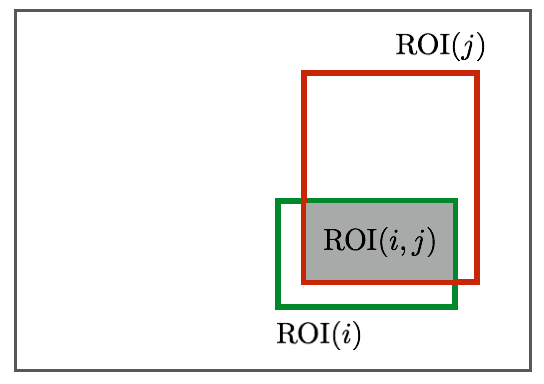
\includegraphics[width=4cm]{figures/weight-define}
    \caption{Weight Definition Visualization}
    \label{fig:roiweight}
    \end{figure}

    For a certain image $img$ at time $t$, Rating: player $i$ $\rightarrow$ player $j$:

    \[
    w_{ij}=\sum_{\text{ROI}\in \text{ROIs}}\frac{\text{ROI}(i,j)}{\text{ROI}(i)} \times \frac{Cov(\text{tags}(i), \text{tags}(j))}{\text{var}(\text{tags}(i))\text{var}(\text{tags}(j))} \geq 0
    \]

    Normalized Adjacency Matrix:

    \[
    A = (\frac{w_{ij}}{\sum_{j}{w_{ij}}})
    \]

    Obviously, A is \textbf{irreducible, real, non-negative, column-stochastic, and diagonal element being positive,} then eigenvalue of A is the player trust value.

    When a new player tagging task need to be rated,

    \begin{itemize}
      \item which means we need introduce a new node to the graph
      \item need calculate the trust value of new graph
      \item let $t’$ is the trust value of new player
      \item if $t’ >= \text{mean}(\text{old\_eigenvalues})$, then it is a reliable player, otherwise drop it.
    \end{itemize}

    \subsubsection{Disaster Level Evaluation Model}

    Query input:

    \[
    (\text{time}) or (\text{area\_id})/(\text{area\_id}, \text{time})
    \]

    Model output:

    \[
    (\text{area\_id}, \text{time}, \text{disaster\_level})
    \]

    Note that:

    \begin{itemize}
      \item All results are evaluated from reliable tasks
      \item Evaluation Model generated by all reliable history
    \end{itemize}

    Now we have trusted results, each area has its tagging history.

    For an area at time t, define disaster level as follows:

    \[
    v_{area} = \frac{
    \sum_{\text{tag}\in\text{tags}}
      {w_{tag}\times\#(\text{tag})}
    }
    {\sum_{area\in areas}{\sum_{\text{tag}\in\text{tags}}{w_{tag}\times\#(\text{tag})}}}
    \]

    where $w_{tag}$ is pre-defined weight by system, $\#(tag)$ is the occur number of a tag.

    Return value:

    \begin{itemize}
      \item disaster region: $\cup_{ROI\in ROIs}{ROI}$
      \item disaster level: $v_{area}$
    \end{itemize}

    \subsubsection{Data Persistence}

    Trusted DB Fields:

    \begin{lstlisting}[
      caption={Trusted Database Field},
      label={lst:trustdb}
    ]
    [
        {
            "anonymous_id": number,
            "tasks": [
                {
                    "image": image_path,
                    "at_time": time, 
                    "ROI": [
                        {
                            "latitude": number,
                            "longitude": number,
                            "tags": [tag1, tag2, ...]
                        }
                    ]
                }
            ]
            "trust_value": number
        }
    ]
    \end{lstlisting}

    Result DB Fields:

    \begin{lstlisting}[
      caption={Results Database Field},
      label={lst:resultdb}
    ]
    [
        {
            “area_id": number,
            "history": [
                {
                    “at_time”: time,
                    "image": image_path,
                    "ROI": [
                        {
                            "latitude": number,
                            “longitude": number,
                            "tags": [tag1, tag2, ...]
                        }
                    ],
                    "disaster_level": number
                }
            ]
        }
    ]
    \end{lstlisting}

